\documentclass{article}
\usepackage[utf8]{inputenc}
\usepackage[english,russian]{babel}

\title{Выделение группы ВУЗов со схожими финансовыми показателями}
\author{Бобкова Анастасия}
\date{Январь 2021}

\usepackage{natbib}
\usepackage{graphicx}

\begin{document}

\maketitle

\newpage
\tableofcontents

\newpage
\section{Введение}
There is a theory which states that if ever anyone discovers exactly what the Universe is for and why it is here, it will instantly disappear and be replaced by something even more bizarre and inexplicable.
There is another theory which states that this has already happened.

\begin{figure}[h!]
\centering
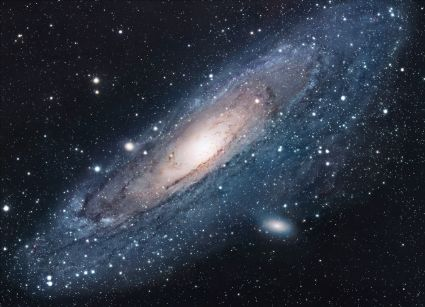
\includegraphics[scale=1.7]{universe}
\caption{The Universe}
\label{fig:universe}
\end{figure}

\section{Данные}
\subsection{Набор данных с названием ВУЗа и его ИНН}
\subsection{Набора данных с ИНН вуза, годом отчета и финансовыми показателями}
\subsection{Очистка данных}

\section{Методы}

\section{Анализ}
\subsection{Вычисление корреляции между финансовыми показателями}
\subsection{Выявление группы ВУЗов, в отчетах которых встречаются аномальные значения}
\subsection{Масштабирование данных}
\subsection{Кластерный анализ}

\section{Результаты}

\section{Заключение}
``I always thought something was fundamentally wrong with the universe'' \citep{adams1995hitchhiker}

\bibliographystyle{plain}
\bibliography{references}
\end{document}
